\documentclass[10pt]{article}

\usepackage[a4paper,margin=2.2cm]{geometry}
\usepackage[T1]{fontenc}
\usepackage[utf8]{inputenc}
\usepackage{lmodern}
\usepackage{microtype}
\usepackage{amsmath,amssymb,mathtools}
\usepackage{booktabs,tabularx,array,multirow}
\usepackage{enumitem}
\usepackage{xcolor}
\usepackage{graphicx}
\usepackage{tikz}
\usetikzlibrary{arrows.meta,positioning,fit,shapes.geometric}
\usepackage{listings}
\usepackage{hyperref}
\usepackage[nameinlink,noabbrev]{cleveref}
\usepackage{caption}
\usepackage{subcaption}
\usepackage{url}
\usepackage{balance}

\definecolor{acmblue}{RGB}{37,80,130}
\definecolor{acmgray}{RGB}{245,247,249}
\hypersetup{
  colorlinks=true,
  linkcolor=acmblue,
  citecolor=acmblue,
  urlcolor=acmblue,
  pdftitle={Agentic Configuration Management},
  pdfauthor={AUTHOR NAME}
}

\lstdefinestyle{acmcode}{
  basicstyle=\ttfamily\small,
  backgroundcolor=\color{acmgray},
  frame=single,
  rulecolor=\color{black!15},
  breaklines=true,
  columns=fullflexible,
  showstringspaces=false
}

\newcommand{\acmcore}{\textsc{ACM Core}}
\newcommand{\framework}{framework-independent}
\newcommand{\todo}[1]{\textcolor{red}{[TODO: #1]}}
\newcommand{\system}{\mathcal{S}}
\newcommand{\configgraph}{G_C}
\newcommand{\runtimegraph}{G_R}
\newcommand{\assurancegraph}{G_A}
\newcommand{\evolutiongraph}{G_E}

\title{\textbf{Agentic Configuration Management (ACM):\\A Reference Configuration Model for Governed Agentic Systems}}

\author{
  AUTHOR NAME\\
  AFFILIATION\\
  \texttt{EMAIL ADDRESS}
}

\date{Draft --- July 2026}

\begin{document}
\maketitle

\begin{abstract}

Agentic systems are rapidly evolving from isolated LLM applications to complex software composed of interacting agents, tools, prompts, models, and execution workflows. While existing LLMOps and AgentOps platforms provide valuable support for orchestration and observability, they do not offer a framework-independent configuration model capable of describing, validating, and governing the system as a coherent whole. As a result, configuration management remains fragmented across frameworks, making reproducibility, impact analysis, and long-term maintenance increasingly difficult.

This paper introduces \textbf{Agentic Configuration Management (ACM)}, a reference configuration model designed for governed agentic systems. ACM extends established Software Configuration Management principles to the agentic domain through immutable configuration items, explicit baselines, lifecycle management, dependency-aware state propagation, and runtime provenance. Rather than replacing existing orchestration frameworks, ACM provides a common representation that enables their configurations to be normalized and managed consistently.

We describe a complete reference implementation in Python together with adapters for LangGraph and CrewAI. The implementation includes a deterministic validation engine, a replayable event model, and a preservation-based extraction process that reconstructs native workflows into the ACM representation. The evaluation combines normative scenarios with automated tests to assess both the consistency of the model and the fidelity of the extraction process across frameworks.

The results show that ACM can preserve the structural information required for configuration governance while making explicit the information that is approximated or unavailable in the underlying framework. These results provide initial evidence that a unified configuration model can support reproducibility, auditability, and governance across heterogeneous agentic ecosystems without being tied to a specific orchestration framework.

\end{abstract}

\section{Introduction}

Large-language-model applications are moving from linear prompt chains toward agentic systems that combine autonomous or semi-autonomous agents, tools, models, policies, memories, and workflow structures. A single deployed system may contain several independently evolving prompts, multiple model profiles, external tools with distinct permissions, stateful execution graphs, evaluation suites, and runtime-created agents. The resulting behavior is determined not by one artifact, but by a \emph{resolved composition} of artifacts and dependencies.

Current engineering practices address parts of this problem. Version-control systems record source-code changes; prompt registries version templates; observability platforms connect traces to prompts and evaluations; orchestration frameworks represent workflows and runtime state. Yet these mechanisms usually answer different questions. A trace describes what occurred during an execution. A prompt registry identifies which prompt was used. A framework object defines how execution is orchestrated. None of these artifacts alone necessarily identifies the complete configuration that was approved, tested, released, and executed.

This fragmentation creates four practical problems.

\begin{enumerate}[leftmargin=*]
  \item \textbf{Composite identity.} There is no common identity for a complete agentic system assembled from independently versioned components.
  \item \textbf{Change impact.} A modified prompt, model, tool, or policy may invalidate evidence or affect multiple upstream agents and workflows, but the impact is rarely computed explicitly.
  \item \textbf{Runtime mutation.} Dynamic agents and runtime graph extensions alter the effective system after release, often without becoming governed configuration artifacts.
  \item \textbf{Framework portability.} Agentic frameworks expose different abstractions, making cross-framework comparison and audit difficult.
\end{enumerate}

Software Configuration Management (SCM) has long addressed analogous concerns for conventional software: configuration-item identification, baselines, change control, status accounting, build and release management, and audits. However, a direct application of conventional SCM is insufficient. Agentic systems include probabilistic components, externally hosted models, generated prompts, runtime graph mutations, and execution-specific instances. They therefore require a configuration model that preserves SCM's integrity principles while explicitly representing these properties.

This paper proposes \emph{Agentic Configuration Management} (ACM), a reference configuration model and lightweight implementation for governed agentic systems. ACM is not an orchestrator, an evaluation platform, or an observability backend. It is a representation, validation, and traceability layer that can complement such tools.

\paragraph{Contributions.}
This paper makes the following contributions:

\begin{itemize}[leftmargin=*]
  \item \textbf{A normative reference model} for representing prompts, agents, workflows, tools, models, policies, evaluation profiles, factories, and systems as versioned Agentic Configuration Items (ACIs).
  \item \textbf{A state and propagation model} separating lifecycle, quality, assurance, impact, and eligibility, with deterministic, non-destructive propagation rules.
  \item \textbf{A runtime governance model} based on normalized events, replayable runtime graphs, controlled dynamic-agent creation, permission ceilings, and explicit drift classification.
  \item \textbf{A Python reference implementation} using strict schemas, canonical digests, fixed-point propagation, state machines, scenario harnesses, and framework adapters.
  \item \textbf{An experimental evaluation} covering 27 scenarios and non-trivial extraction experiments for LangGraph and CrewAI.
\end{itemize}

The remainder of the paper first positions ACM relative to SCM, prompt management, LLMOps/AgentOps, and agent frameworks. It then presents the design goals, reference model, runtime model, framework projections, implementation, evaluation, limitations, and future work.

\section{Background and Related Work}
\label{sec:related}

\subsection{Software Configuration Management}

SCM is concerned with preserving product integrity while software evolves. Its core functions include configuration identification, change control, configuration status accounting, audits, build management, and release management~\cite{ieee828,swebok2024}. A configuration item is an artifact selected for independent control; a baseline is an approved configuration serving as a reference for subsequent change.

ACM adopts these principles but changes the unit of management. In conventional software, source files, libraries, deployment descriptors, and binaries may be configuration items. In an agentic system, relevant items also include prompts, agent definitions, model profiles, tool interfaces, policies, evaluation profiles, workflow topologies, and runtime factories. Moreover, a released configuration may produce runtime instances that were not present as permanent objects at design time.

Git contributes content-addressed objects, immutable commits, history, and references~\cite{gitinternals}. However, Git does not understand the domain semantics of an agent, a prompt, a permission ceiling, an assurance profile, or a runtime delegation. ACM therefore treats Git as a possible storage substrate rather than as the configuration model itself.

\subsection{Prompt Management and LLMOps}

Prompt-management systems commonly provide registries, versions, deployment labels, diffs, evaluation links, and rollbacks. LLM observability platforms add traces, costs, latency, datasets, and feedback. These capabilities are essential but typically prompt-centered or execution-centered. They do not necessarily define a composite identity for the full agentic system or propagate the effect of a component change through a dependency graph.

MLflow, LangSmith, Langfuse, PromptLayer, Weights \& Biases Weave, Braintrust, Helicone, Promptfoo, and related systems cover overlapping combinations of prompt registration, evaluation, tracing, and deployment. The relevant gap is not an absence of versioning or observability. It is the absence of a common model that combines exact component revisions, baseline resolution, lifecycle decisions, assurance evidence, runtime mutation, and dependency-aware eligibility for a complete agentic system.

\subsection{Agent Frameworks}

Agent frameworks expose heterogeneous abstractions. LangGraph represents explicit stateful graphs with nodes, edges, conditional transitions, and checkpoints. CrewAI distinguishes role- and task-oriented Crews from event-driven Flows. Other ecosystems emphasize handoffs, conversations, typed workflows, pipelines, or hierarchical agent structures.

Frameworks generally focus on execution. Their persisted state answers where an execution was and how it can resume. Their traces answer which operations occurred. These are distinct from configuration questions such as which exact revisions were approved, which evidence applies, whether a dependency change makes a composite stale, or whether a runtime-created agent exceeded its declared permission ceiling.

\subsection{Research Gap}

The literature and industrial tooling reviewed for this work provide many of the required building blocks, but no examined approach combines all of the following in a single framework-independent model:

\begin{itemize}[leftmargin=*]
  \item typed and independently versioned agentic configuration items;
  \item exact revision identities and content digests;
  \item immutable, fully resolved release baselines;
  \item explicit lifecycle and release state machines;
  \item assurance evidence linked to exact revisions and dependency snapshots;
  \item deterministic impact and eligibility propagation;
  \item runtime graph reconstruction from normalized events;
  \item governed runtime-created agents and permission ceilings; and
  \item extraction into a common intermediate representation across distinct frameworks.
\end{itemize}

ACM is intended to fill this systems-engineering gap rather than replace existing orchestration, tracing, or evaluation tools.

\section{Design Goals}
\label{sec:goals}

The design is guided by six goals.

\paragraph{G1: Framework portability.}
The core representation must not depend on native LangGraph, CrewAI, or other framework classes. Framework-specific logic is confined to adapters and extractors.

\paragraph{G2: Exact configuration identity.}
A released configuration must resolve all moving references to exact revisions and include content digests sufficient to detect later mutation.

\paragraph{G3: Non-destructive state semantics.}
A failing dependency may block a composite's promotion without overwriting the composite's intrinsic quality judgment. Intrinsic and computed states must remain distinct.

\paragraph{G4: Deterministic reasoning.}
Given the same graph, evidence, and policy, state propagation and replay must produce the same normalized results regardless of input ordering.

\paragraph{G5: Runtime accountability.}
Runtime-created agents and graph mutations must be traceable to approved definitions, factories, overrides, permissions, and events.

\paragraph{G6: Lightweight implementation.}
The reference implementation must run locally without a distributed database, GPU, or orchestration platform. It should support small and medium-sized configurations and serve as an executable specification.

\section{ACM Reference Model}
\label{sec:model}

\subsection{Agentic Configuration Items}

An \emph{Agentic Configuration Item} (ACI) is an independently identifiable and versioned unit of an agentic system. ACM Core defines the following primary kinds:

\begin{itemize}[leftmargin=*]
  \item \texttt{AgenticSystem};
  \item \texttt{WorkflowDefinition};
  \item \texttt{AgentDefinition};
  \item \texttt{PromptDefinition};
  \item \texttt{ToolDefinition};
  \item \texttt{ModelProfile};
  \item \texttt{PolicyDefinition};
  \item \texttt{AgentFactoryDefinition};
  \item \texttt{EvaluationProfile}; and
  \item \texttt{ReleaseBaseline}.
\end{itemize}

Each ordinary ACI revision contains a stable logical identifier, a unique revision identifier, a semantic version, timestamps, provenance, intrinsic states, type-specific content, and a cryptographic digest.

\begin{lstlisting}[style=acmcode,caption={Simplified ACI revision.}]
{
  "kind": "AgentDefinition",
  "id": "aci:agent:planner",
  "version": "1.0.0",
  "revision_id": "01J...",
  "lifecycle_state": "validated",
  "quality_state": "ok",
  "assurance_state": "assessed",
  "content": { ... },
  "provenance": { ... },
  "digest": {"algorithm": "sha256", "value": "..."}
}
\end{lstlisting}

The logical \texttt{id} persists across revisions. The \texttt{revision\_id} identifies one exact revision. The digest binds canonicalized content and references. This separation supports lineage, exact evidence targeting, and tamper detection.

\subsection{Four Interconnected Graphs}

ACM separates four modeling spaces rather than treating all relations as one undifferentiated graph:

\begin{align}
  \configgraph &= (V_C,E_C) && \text{configuration composition and dependencies},\\
  \evolutiongraph &= (V_E,E_E) && \text{revision lineage and replacement},\\
  \runtimegraph &= (V_R,E_R) && \text{runtime instances and observed interactions},\\
  \assurancegraph &= (V_A,E_A) && \text{evidence, evaluations, and approvals}.
\end{align}

The graphs may share identifiers, but each relation type belongs to one modeling space. For example, an agent may \texttt{uses\_prompt} in $\configgraph$, be \texttt{derived\_from} another revision in $\evolutiongraph$, \texttt{invokes} a tool in $\runtimegraph$, and be \texttt{validated\_by} evidence in $\assurancegraph$. This separation of concerns is stronger and more defensible than claiming that relation families are mathematically orthogonal.

\begin{figure}[t]
\centering
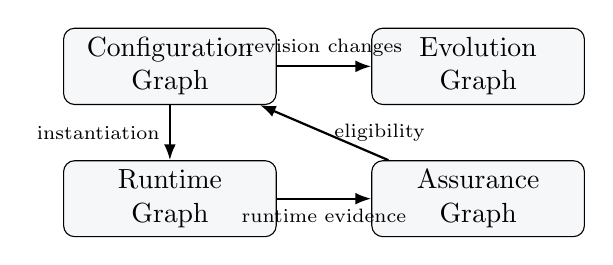
\begin{tikzpicture}[
  node distance=7mm and 12mm,
  box/.style={draw,rounded corners,align=center,minimum width=27mm,minimum height=9mm,fill=acmgray},
  arrow/.style={-{Latex[length=2mm]},thick}
]
\node[box] (config) {Configuration\\Graph};
\node[box,right=of config] (evol) {Evolution\\Graph};
\node[box,below=of config] (runtime) {Runtime\\Graph};
\node[box,right=of runtime] (assure) {Assurance\\Graph};
\draw[arrow] (config) -- node[above,sloped,font=\scriptsize]{revision changes} (evol);
\draw[arrow] (config) -- node[left,font=\scriptsize]{instantiation} (runtime);
\draw[arrow] (assure) -- node[right,font=\scriptsize]{eligibility} (config);
\draw[arrow] (runtime) -- node[below,sloped,font=\scriptsize]{runtime evidence} (assure);
\end{tikzpicture}
\caption{ACM separates configuration, evolution, runtime, and assurance concerns while allowing cross-graph references.}
\label{fig:fourgraphs}
\end{figure}

\subsection{Release Baselines}

A \texttt{ReleaseBaseline} is an exact snapshot of a resolved configuration. It contains exact ACI revision references, relations, validation results, provenance, and a baseline digest. A released baseline is logically immutable: changing its content causes digest verification to fail. The reference implementation is therefore \emph{tamper-evident}, not physically append-only.

A baseline lifecycle is distinct from the ACI lifecycle:

\[
\texttt{candidate} \rightarrow \texttt{released} \rightarrow \{\texttt{superseded},\texttt{withdrawn}\}.
\]

A baseline may be released only if all mandatory references resolve exactly, the baseline digest is valid, required items are validated, required evidence is complete, and no mandatory component is blocked by policy.

\subsection{Lifecycle State Machines}

ACI revisions use the normative states:

\[
\texttt{draft},\ \texttt{candidate},\ \texttt{validated},\ \texttt{deprecated},\ \texttt{archived}.
\]

The principal allowed transitions are:

\begin{align*}
\texttt{draft} &\rightarrow \texttt{candidate},\\
\texttt{candidate} &\rightarrow \texttt{draft},\\
\texttt{candidate} &\rightarrow \texttt{validated},\\
\texttt{validated} &\rightarrow \texttt{deprecated},\\
\texttt{deprecated} &\rightarrow \texttt{archived}.
\end{align*}

An archived or deprecated revision is not reactivated in place; a new revision is required. This rule preserves historical semantics and avoids rewriting the lifecycle of previously identified content.

\subsection{Intrinsic and Computed States}

ACM deliberately separates intrinsic states from graph-derived states.

\paragraph{Intrinsic states.}
These are attached to one exact revision:

\[
\texttt{lifecycle\_state},\quad
\texttt{quality\_state},\quad
\texttt{assurance\_state}.
\]

\paragraph{Computed states.}
These are recalculated from graph structure, evidence, and policy:

\[
\texttt{impact\_state},\quad
\texttt{eligibility\_state},\quad
\texttt{effective\_quality},\quad
\texttt{effective\_assurance}.
\]

A tool with intrinsic quality \texttt{nok} may make a dependent agent \texttt{blocked} for promotion. It does not automatically rewrite the agent's intrinsic quality to \texttt{nok}. This non-destructive approach preserves the source of each judgment.

\subsection{Assurance Evidence}

Evidence targets an exact revision and digest. It also records scope dimensions, environment constraints, result, blocking status, validity interval, producer, and a dependency snapshot. Let $R(x)$ be the required applicable checks for revision $x$, and $E(x)$ the subset with valid evidence. Assurance coverage is:

\begin{equation}
\operatorname{coverage}(x)=
\begin{cases}
1, & |R(x)|=0,\\
\dfrac{|E(x)|}{|R(x)|}, & \text{otherwise.}
\end{cases}
\end{equation}

The assurance state is then:

\begin{equation}
A(x)=
\begin{cases}
\texttt{unassessed}, & \operatorname{coverage}(x)=0,\\
\texttt{partially\_assessed}, & 0<\operatorname{coverage}(x)<1,\\
\texttt{assessed}, & \operatorname{coverage}(x)=1.
\end{cases}
\end{equation}

Coverage represents completeness, not success. Thus \texttt{quality=nok} and \texttt{assurance=assessed} is a valid and important combination: the required evaluation was complete and revealed a failure.

Evidence is non-transitive by default. A workflow-level evaluation does not automatically validate every contained agent unless the scope explicitly includes those revisions and the applicable policy allows composition.

\subsection{Impact and Eligibility Propagation}

Impact and eligibility are propagated according to typed dependency relations and project policy. Impact states are ordered:

\[
\texttt{current} < \texttt{impacted} < \texttt{stale}.
\]

An ACI becomes \texttt{impacted} when a relevant dependency changes or a policy indicates potential effect. It becomes \texttt{stale} when previously applicable evidence no longer matches the revision, digest, environment, or dependency snapshot.

Eligibility is context-dependent and uses values such as:

\[
\texttt{eligible},\quad \texttt{warning},\quad \texttt{blocked}.
\]

Examples of blocking conditions include unresolved mandatory references, a mandatory dependency with effective quality \texttt{nok}, a forbidden runtime override, permission escalation, or a withdrawn baseline.

The propagation engine computes a fixed point. Abstractly, with configuration $C$, evidence $E$, and policy $P$:

\begin{equation}
\operatorname{status}^{*}=\operatorname{lfp}\left(F_{C,E,P}\right),
\end{equation}

where $F$ updates assurance, impact, effective quality, and eligibility until no normalized state changes. Deterministic ordering and monotone severity aggregation are used where applicable.

\section{Runtime Model}
\label{sec:runtime}

\subsection{Normalized Runtime Events}

Framework adapters emit normalized runtime events instead of passing native framework objects into the ACM core. Primitive events include instance creation, state transitions, relation creation, configuration resolution, tool invocation, delegation, termination, and validation results. Composite events may summarize a higher-level operation but must remain reducible to primitive events when replay is required.

The runtime graph at time $t$ is reconstructed from a released baseline $G_B$ and an ordered event sequence:

\begin{equation}
G_t=\operatorname{replay}(G_B,e_1,e_2,\ldots,e_t).
\end{equation}

Replay determinism applies to normalized graph state and digests, excluding non-semantic metadata such as randomly generated report identifiers or report-generation timestamps.

\subsection{Runtime State Machine}

Runtime instances use:

\[
\texttt{created},\ \texttt{ready},\ \texttt{running},\ \texttt{waiting},\ \texttt{completed},\ \texttt{failed},\ \texttt{cancelled},\ \texttt{terminated}.
\]

Invalid transitions are rejected at event append time in strict mode. For example, a transition from \texttt{completed} back to \texttt{running} is invalid. Rejecting malformed transitions preserves the integrity of the append log and avoids allowing replay to construct impossible states.

\subsection{Dynamic Agents}

ACM distinguishes an \texttt{AgentDefinition} from an \texttt{AgentInstance}. A dynamic instance must reference an approved definition or factory, record its creator and execution, resolve its model, prompts, tools, policies, permissions, and overrides, and receive a configuration digest.

An \texttt{AgentFactoryDefinition} specifies:

\begin{itemize}[leftmargin=*]
  \item allowed templates;
  \item fields that may be overridden;
  \item model and tool allowlists;
  \item permission ceilings;
  \item delegation depth and instance limits; and
  \item runtime lifetime.
\end{itemize}

The core safety invariant is:

\begin{equation}
\operatorname{permissions}(child) \subseteq \operatorname{ceiling}(factory)
\subseteq \operatorname{permissions}(creator),
\end{equation}

unless a more restrictive project policy is configured. Forbidden overrides, such as unauthorized tools, models, policies, or permissions, produce \texttt{blocked} eligibility.

Runtime-created objects follow a separate promotion machine:

\[
\texttt{ephemeral}\rightarrow\texttt{retained}\rightarrow\texttt{candidate}\rightarrow\texttt{registered}.
\]

A runtime object cannot be promoted directly from ephemeral to registered, and registration creates a new ordinary ACI revision rather than modifying the release baseline that produced the run.

\subsection{Configuration Drift}

ACM distinguishes several concepts that are often conflated under \emph{drift}:

\begin{itemize}[leftmargin=*]
  \item \textbf{declared extension}: a runtime instance or relation was allowed by the baseline and factory policy;
  \item \textbf{undeclared instance}: a runtime element has no valid traceability path to an approved definition or factory;
  \item \textbf{configuration mismatch}: the resolved configuration differs from the declared or expected configuration;
  \item \textbf{withdrawn baseline use}: a run references a baseline that has been explicitly withdrawn.
\end{itemize}

The reference engine keeps a compact drift state while the evaluation harness derives more explanatory classifications. This is an acknowledged model refinement rather than an unreported mismatch.

\section{Framework Projection}
\label{sec:projection}

\subsection{Intermediate Representation}

Framework extraction maps native objects to a canonical workflow intermediate representation (IR). The IR records nodes, direct edges, conditional branches, entry and terminal nodes, agent references, prompt references, tool references, state schema, extraction status, unresolved elements, and canonical digests.

Each extracted property is classified as:

\begin{itemize}[leftmargin=*]
  \item \texttt{preserved}: reconstructed exactly within the ACM scope;
  \item \texttt{approximated}: represented at the ACM abstraction level, but with opaque native semantics; or
  \item \texttt{unsupported}: no ACM mapping is currently available.
\end{itemize}

Nodes may also be marked \texttt{extracted}, \texttt{declared\_by\_adapter}, or \texttt{unresolved}. This distinction prevents adapter-supplied metadata from being misrepresented as native discovery.

\subsection{LangGraph Mapping}

The LangGraph extractor reads explicit topology, including nodes, direct edges, branch targets, entry points, and terminal nodes. ACM-specific semantic references such as agent, prompt, model, and tool identities can be supplied through explicit node metadata when they are not recoverable from the graph object itself.

For the evaluated non-trivial workflow, the latest report records 100\% node, relation, and branch coverage; entry and terminal preservation; 100\% prompt and tool references; stable repeated-extraction digests; and one approximated property: the internal semantics of conditional routing functions remain opaque.

This supports the claim that explicit LangGraph topology is structurally extractable for the studied case. It does not imply that arbitrary Python branch logic can be semantically interpreted.

\subsection{CrewAI Mapping}

CrewAI requires separate handling of Crews and Flows. Crew extraction identifies agents, tasks, context dependencies, tools, and process information. Flow extraction identifies start methods, routers, listeners, branches, state, and termination paths. A combined Flow+Crew projection merges orchestration topology with role/task semantics.

A true non-trivial CrewAI Flow has now been added to the reference repository. However, the latest generated preservation report still invokes the earlier Crew-only extraction path while comparing it against a Flow+Crew golden representation. Its reported 42.9\% node coverage, 28.6\% relation coverage, and 0\% branch coverage therefore do not measure the newly implemented Flow. We intentionally do not use those values as evidence of final CrewAI preservation.

The final paper version should replace this paragraph with regenerated Flow+Crew metrics after the report generator is updated. Until then, the defensible claim is limited to: (i) CrewAI Flow extraction is implemented and unit-tested; and (ii) cross-framework normalization evidence remains provisional.

\section{Reference Implementation}
\label{sec:implementation}

The implementation targets Python 3.11--3.13 and uses Pydantic v2 for strict data contracts. Optional dependencies provide Hypothesis, LangGraph, and CrewAI support. The inspected repository contains approximately 11,940 lines of Python across the core, adapters, harness, scenarios, and tests, with 25 Python modules under the \texttt{acm} package and 27 test files.

\subsection{Architecture}

The main modules are:

\begin{itemize}[leftmargin=*]
  \item \texttt{acm.models}: ACI revisions, graphs, relations, baselines, evidence, and runtime objects;
  \item \texttt{acm.propagation}: assurance, quality, impact, eligibility, and fixed-point computation;
  \item \texttt{acm.state\_machines}: lifecycle, baseline, runtime, and promotion transitions;
  \item \texttt{acm.runtime}: event log, replay, dynamic instances, and drift;
  \item \texttt{acm.invariants}: executable invariants;
  \item \texttt{adapters}: framework instantiation and extraction;
  \item \texttt{harness}: scenario loading, assertions, workflow IR, preservation analysis, and reporting; and
  \item \texttt{scenarios}: canonical configurations, native workflows, and case studies.
\end{itemize}

\begin{figure}[t]
\centering
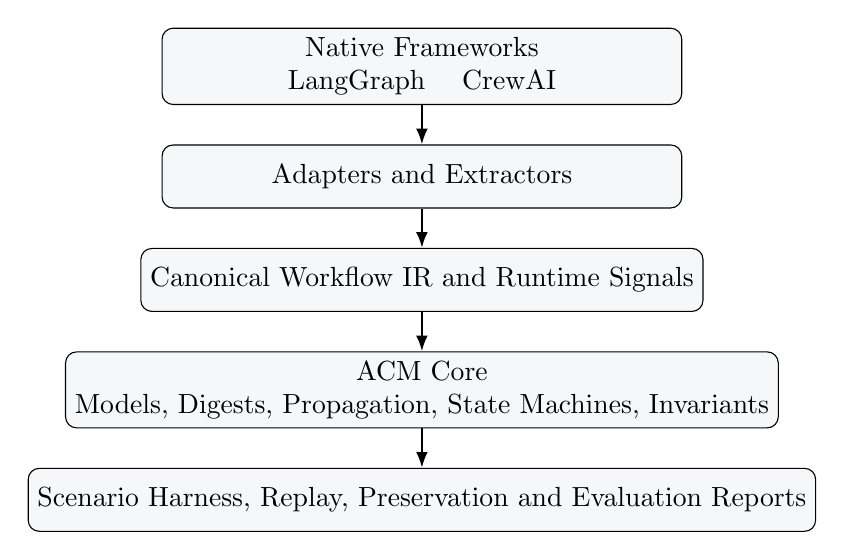
\begin{tikzpicture}[
  node distance=5mm,
  layer/.style={draw,rounded corners,align=center,minimum width=66mm,minimum height=8mm,fill=acmgray},
  arrow/.style={-{Latex[length=2mm]},thick}
]
\node[layer] (frameworks) {Native Frameworks\\LangGraph \quad CrewAI};
\node[layer,below=of frameworks] (adapters) {Adapters and Extractors};
\node[layer,below=of adapters] (ir) {Canonical Workflow IR and Runtime Signals};
\node[layer,below=of ir] (core) {ACM Core\\Models, Digests, Propagation, State Machines, Invariants};
\node[layer,below=of core] (reports) {Scenario Harness, Replay, Preservation and Evaluation Reports};
\draw[arrow] (frameworks)--(adapters);
\draw[arrow] (adapters)--(ir);
\draw[arrow] (ir)--(core);
\draw[arrow] (core)--(reports);
\end{tikzpicture}
\caption{Reference implementation architecture. Native framework objects are confined to adapters.}
\label{fig:architecture}
\end{figure}

\subsection{Canonicalization and Digests}

Configuration and evidence digests are calculated from canonical normalized representations. Semantic fields are included; non-semantic report metadata is excluded. Stable digests support exact evidence matching, repeated-extraction comparison, and tamper detection.

\subsection{Executable Invariants}

The implementation encodes invariants covering exact revision identity, baseline integrity, evidence applicability, non-transitive assurance, deterministic propagation, valid state transitions, runtime provenance, permission ceilings, and controlled promotion. The evaluation scenarios reference these invariants directly.

\section{Experimental Evaluation}
\label{sec:evaluation}

\subsection{Research Questions}

The evaluation addresses four research questions.

\begin{description}[leftmargin=12mm,style=nextline]
  \item[RQ1:] Can ACM represent and validate the core configuration, lifecycle, baseline, assurance, and runtime rules defined by the specification?
  \item[RQ2:] Does the propagation and replay machinery satisfy determinism, convergence, ordering invariance, and the selected invariants?
  \item[RQ3:] Can non-trivial native workflows be extracted into a common ACM representation without silently losing information?
  \item[RQ4:] What local computational cost is observed for small and medium-sized configuration graphs?
\end{description}

\subsection{Evaluation Setup}

The latest complete generated report was produced on Linux x86\_64 with Python 3.13.14, LangGraph and CrewAI installed. It reports 277 passed tests, zero failures, and zero skips. Twenty-seven scenarios are mapped to one or more tests. Eleven propagation scenarios are additionally represented as declarative YAML fixtures and measured through a common harness.

The scenario groups are:

\begin{enumerate}[leftmargin=*]
  \item configuration and baseline integrity (S01--S04);
  \item propagation and assurance (S05--S11);
  \item runtime, replay, and drift (S12--S17);
  \item dynamic agents and permissions (S18--S21); and
  \item portability and robustness (S22--S27).
\end{enumerate}

\subsection{Scenario Results}

\begin{table}[t]
\centering
\caption{Consolidated scenario evaluation.}
\label{tab:scenario-results}
\begin{tabularx}{\linewidth}{lrrrX}
\toprule
Group & Scenarios & Pass & Deviation & Main concerns \\
\midrule
A & 4 & 4 & 0 & Baselines, references, digests, tamper evidence \\
B & 7 & 7 & 0 & Quality, assurance, impact, eligibility \\
C & 6 & 3 & 3 & Replay, transitions, drift taxonomy \\
D & 4 & 4 & 0 & Dynamic agents, permissions, overrides, promotion \\
E & 6 & 6 & 0 & Portability, ordering, cycles, local scale \\
\midrule
Total & 27 & 24 & 3 & No failures or skips \\
\bottomrule
\end{tabularx}
\end{table}

All scenarios pass their executable tests. Three runtime/drift scenarios are classified as \texttt{pass\_with\_deviation}: their detailed labels are derived by the conformity layer rather than represented as first-order values in the compact engine enumeration. These deviations are documented and do not correspond to test failures.

The eleven declarative propagation fixtures converge in one to three iterations, with measured execution times below 1~ms in the reported environment. These timings concern small synthetic fixtures and should not be interpreted as general performance results.

\subsection{Property-Based and Robustness Tests}

Property-based tests cover convergence, idempotence, ordering invariance, and monotone behavior under relevant severity updates. Dedicated tests cover dependency cycles, evidence composition modes, absent versus empty policy semantics, digest sensitivity, invalid runtime transitions, replay, and baseline mutation detection.

The results support deterministic normalized behavior for the tested input domains. They do not constitute a proof for all possible graphs or policy languages.

\subsection{Information Preservation}

The extraction oracle compares native workflow extraction $E(F)$ to a manually defined golden representation over ACM's normative extraction scope.

\paragraph{LangGraph.}
For the evaluated workflow, all structural nodes, relations, branches, entry points, and terminal nodes are preserved. Conditional function semantics are approximated because arbitrary Python functions remain opaque. Semantic references supplied through adapter metadata are explicitly distinguished from native extraction.

\paragraph{CrewAI.}
The repository now includes a real CrewAI Flow and dedicated extraction tests. Final Flow+Crew preservation metrics are pending regeneration because the current reporting script still evaluates the earlier Crew-only object. Consequently, no final cross-framework equivalence percentage is claimed in this draft.

\subsection{Local Scalability}

A prior local benchmark reported approximately 92~ms for 100 ACIs and 300 relations and approximately 8.1~s for 1,000 ACIs and 3,000 relations. The observed growth reflects repeated relation scans inside the fixed-point implementation. The current prototype is therefore suitable for local small- and medium-sized configurations, not for an enterprise-scale registry.

Pre-indexing incoming and outgoing relations by source, target, and type should reduce repeated graph scans and is part of future optimization work.

\subsection{Answers to the Research Questions}

\paragraph{RQ1.}
The 27 scenario suite provides executable evidence that the implemented model covers the intended core behaviors, including exact revisions, baselines, state propagation, assurance, replay, dynamic agents, and permissions.

\paragraph{RQ2.}
The tested implementation converges and produces ordering-invariant normalized states for the covered cases. Runtime transitions are validated at append time, and replay reconstructs the same semantic graph state for the same ordered event log.

\paragraph{RQ3.}
The LangGraph case demonstrates strong structural preservation for an explicit graph. CrewAI Flow extraction is implemented, but the final preservation report must be regenerated before making a quantitative cross-framework claim.

\paragraph{RQ4.}
The implementation is practical for local validation of modest configurations. Its current graph traversal strategy is not yet suitable for large enterprise graphs without indexing and incremental recomputation.

\section{Discussion}
\label{sec:discussion}

\subsection{What ACM Adds}

ACM's main contribution is not a new orchestration runtime. It is a common configuration and governance vocabulary that links design-time configuration, release decisions, evaluation evidence, runtime mutation, and audit. It makes explicit several distinctions that are often collapsed in existing systems:

\begin{itemize}[leftmargin=*]
  \item trace versus configuration;
  \item logical identity versus exact revision;
  \item version versus release baseline;
  \item quality versus assurance completeness;
  \item intrinsic state versus computed eligibility;
  \item declared graph versus runtime graph;
  \item dynamic definition versus runtime instance; and
  \item permitted extension versus undeclared drift.
\end{itemize}

These distinctions allow systems to remain explainable when configuration and runtime behavior evolve independently.

\subsection{Why a Reference Model Rather Than Another Framework}

A new orchestration framework would add one more native representation. ACM instead targets interoperability between frameworks and operational tools. The core can be backed by JSON, JSONL, Git, an artifact store, or a database. It can consume evidence from evaluation platforms and runtime signals from tracing systems. This architectural role is closer to a domain-specific configuration model and executable specification than to an agent runtime.

\subsection{Industrial Applicability}

Potential applications include release manifests for agentic systems, impact analysis after prompt or tool changes, audit trails for dynamic delegation, policy checks for permission escalation, reproducibility records for regulated deployments, and integration with software supply-chain attestations. Real deployment would require stronger persistence, access control, signing, secret management, and distributed coordination than the current prototype provides.

\section{Threats to Validity}
\label{sec:threats}

\paragraph{Construct validity.}
The 27 scenarios operationalize the current ACM specification and may omit relevant real-world failure modes. Passing them demonstrates consistency with the chosen model, not completeness of the model itself.

\paragraph{Internal validity.}
Many tests and goldens were developed alongside the implementation, creating a risk of shared assumptions. Declarative fixtures, property-based tests, independent extraction goldens, and generated reports reduce but do not eliminate this risk.

\paragraph{External validity.}
Only LangGraph and CrewAI are currently included. They represent two distinct orchestration styles, but they cannot establish universal framework independence. Other paradigms, including handoff-centric, conversational, data-pipeline, and distributed multi-agent frameworks, remain untested.

\paragraph{Extraction validity.}
Adapter-provided metadata may supplement information not recoverable from native framework objects. The implementation records this distinction, but preservation percentages remain sensitive to the chosen normative scope and golden representation.

\paragraph{Performance validity.}
The scalability measurements are local synthetic benchmarks on one implementation and environment. They should not be generalized to distributed production registries.

\paragraph{Evidence validity.}
The implementation verifies configuration identity and evaluation coverage, but it cannot guarantee semantic reproducibility of remote probabilistic models or future availability of external services.

\section{Future Work}
\label{sec:future}

Immediate work is divided into two deferred priorities.

\paragraph{P1: extraction robustness.}
Planned work includes explicit tests for task-identifier collisions, duplicate agent roles, permutation stability, unsupported-element reporting, and additional non-trivial workflow variations. This priority also includes finalizing the Flow+Crew preservation report and formalizing information loss as a first-class extraction result.

\paragraph{P2: projection and scale.}
Longer-term work includes round-trip projection, ACM-to-framework construction, incremental propagation, relation indexes, append-only or signed persistence, framework-version matrices, distributed event logs, and larger performance studies.

Additional adapters may target Microsoft Agent Framework, Google ADK, OpenAI Agents SDK, or Haystack. A third framework is deliberately not required for the present article; broader architectural coverage is reserved for future work.

Other extensions include OpenTelemetry semantic conventions, AI/agent bills of materials, signed attestations, deployment-state objects, policy-as-code integration, and formal verification of selected invariants.

\section{Conclusion}

This paper introduced Agentic Configuration Management, a reference model for identifying, validating, releasing, and auditing composite agentic systems. ACM extends Software Configuration Management with typed agentic configuration items, exact revision identities, tamper-evident baselines, separated intrinsic and computed states, assurance evidence, deterministic propagation, replayable runtime graphs, and controlled dynamic agents.

The Python reference implementation demonstrates that the model is implementable as a lightweight local layer. Its 27-scenario evaluation and 277 passing tests provide evidence for the consistency of the current core. The LangGraph extraction case shows complete structural preservation over the evaluated scope. CrewAI Flow extraction is implemented but awaits corrected report generation before quantitative preservation claims are finalized.

ACM is not yet a production configuration service, nor does it prove universal framework independence. It provides a concrete, executable foundation on which stronger reproducibility, governance, auditability, and interoperability mechanisms for agentic systems can be built.

\section*{Artifact Availability}

The reference implementation, scenarios, and generated reports will be made available at:

\begin{center}
\url{REPOSITORY_URL}
\end{center}

\todo{Replace author, affiliation, email, repository URL, and final CrewAI preservation metrics before submission.}

\bibliographystyle{plain}
\bibliography{references}

\appendix

\section{Scenario Catalogue}
\label{app:scenarios}

\begin{table}[h]
\centering
\caption{Evaluation scenarios.}
\begin{tabularx}{\linewidth}{llX}
\toprule
ID & Priority & Purpose \\
\midrule
S01 & P0 & Nominal configuration and promotion \\
S02 & P0 & Missing mandatory reference \\
S03 & P0 & Exact evidence identity and digest matching \\
S04 & P0 & Released-baseline tamper detection \\
S05 & P0 & Blocking dependency with NOK quality \\
S06 & P1 & Non-blocking dependency warning \\
S07 & P0 & New prompt revision and evidence invalidation \\
S08 & P0 & Distributed assurance coverage \\
S09 & P0 & Complete evidence with failing result \\
S10 & P0 & Direct, aggregate, and hybrid assurance modes \\
S11 & P0 & Missing versus explicitly empty policy \\
S12 & P0 & Deterministic nominal replay \\
S13 & P0 & Invalid runtime state transition \\
S14 & P0 & Authorized runtime mutation \\
S15 & P0 & Undeclared runtime instance \\
S16 & P1 & Prompt configuration mismatch \\
S17 & P1 & Baseline withdrawn after a historical run \\
S18 & P0 & Conforming dynamic agent \\
S19 & P0 & Permission escalation rejected \\
S20 & P1 & Forbidden behavioral override \\
S21 & P1 & Promotion of a runtime-created agent \\
S22 & P0 & Equivalent system in LangGraph and CrewAI \\
S23 & P1 & Explicit versus distributed topology \\
S24 & P1 & Runtime event equivalence \\
S25 & P0 & Input-order invariance \\
S26 & P1 & Dependency cycles \\
S27 & P2 & Local volume and scalability \\
\bottomrule
\end{tabularx}
\end{table}

\section{Submission Checklist}

Before submission, the following items must be updated:

\begin{itemize}[leftmargin=*]
  \item author identity, affiliation, email, and acknowledgments;
  \item repository URL and archival artifact DOI, if available;
  \item regenerated CrewAI Flow+Crew preservation metrics;
  \item exact dependency versions or a lockfile reference;
  \item final bibliographic verification and BibTeX normalization;
  \item final benchmark hardware description;
  \item disclosure of AI assistance according to the target venue's policy; and
  \item replacement of all red TODO markers.
\end{itemize}

\end{document}
